\chapter{Proposed Solutions}

\section{Tools used}
\subsection{3D Slicer}
\textbf{Slicer}, or \textbf{3D Slicer}, is a free, open source software package for visualization and image analysis. It is natively designed to be available on multiple platforms, including Windows, Linux and Mac Os X.

3D Slicer provides image registration, processing of DTI (diffusion tractography), an interface to external devices for image guidance support, and GPU-enabled volume rendering, among other capabilities. 3D Slicer has a modular organization that allows the easy addition of new functionality and provides a number of generic features not available in competing tools.

3D Slicer is built on VTK, a pipeline-based graphical library that is widely used in scientific visualization. In version 4, the core application is implemented in C++, and the API is available through a Python wrapper to facilitate rapid, iterative development and visualization in the included Python console. The user interface is implemented in Qt, and may be extended using either C++ or Python.

Slicer supports several types of modular development. Fully interactive, custom interfaces may be written in C++ or Python. Command-line programs in any language may be wrapped using a light-weight XML specification, from which a graphical interface is automatically generated \cite{slicer}.

For more information on this tool please refer to its official webpage: 

\url{http://www.slicer.org/}

\subsection{ITK}
ITK stands for \textbf{Insight Segmentation and Registration Toolkit}, it's a cross-platform, open-source application development framework widely used for the development of image segmentation and image registration programs.

ITK  is implemented in C++ and it is wrapped for Tcl, Python and Java. This enables developers to create software using a variety of programming languages.

ITK's code is highly efficient, which means that many software problems are discovered at compile-time, rather than at run-time during program execution. It also enables ITK to work on two, three, four or more dimensions.

For more information on this tool please refer to its official webpage: 

\url{http://www.itk.org/}

\subsection{Other Tools}
\subsubsection{Programming Languages}
The programming languages chosen during this project are \textbf{C++} and \textbf{Python}, mainly because they are main languages in which 3D Slicer is written, which means that it was easier to communicate with 3D Slicer by using them.

\subsubsection{MATLAB}
MATLAB is a numerical computing environment and programming language. It allows matrix manipulations, plotting of functions and data, implementation of algorithms, creation of user interfaces, and interfacing with programs written in other languages, including C, C++, Java, and Fortran \cite{matlab}.

MATLAB was used during this project specifically to create and quickly manipulate MRI volume files.

Official website for this tool: \url{http://www.mathworks.com/}

\subsubsection{ParaView}
ParaView is an open-source, multi-platform data analysis and visualization application. ParaView users can quickly build visualizations to analyze their data using qualitative and quantitative techniques.

ParaView was used during this project to visualize the deformation fields produced after the registration of two volumes.

Official website for this tool: \url{http://www.paraview.org/}

\section{Implemented Methods}
During the course of this project two different methods where
implemented, both taking into account previous works about morphometry
and quantification of small changes in volumes.

\subsection{Voxel-based method}
This method was implemented as a \textit{3D Slicer} module with the following steps:
\begin{enumerate}
\item The user selects the base and follow-up volumes to be compared.
\item The user selects the registration method to be used and applies it on the volumes.
\item The module subtracts the base volume and the volume resulting
  from the registration and shows the resulting differences as colored
  layer on top of the base volume.
\end{enumerate}

The registration methods available are: \textit{Affine registration}
(default), \textit{B-Spline deformable registration} and
\textit{BRAINS Demon Warp registration}; all of them available as
already existing modules in \textit{3D Slicer}.

For more information on the registration methods, please refer to
section~\ref{sec:reg_methods}.\\

The subtraction is done pixel-by-pixel and the result produces a label
volume that shows the differences in color over the original base
volume. The chosen color table for the label volume is ``PET-Heat'',
directly available in \textit{3D Slicer}, since it seemed to produce a
volume that was brighter and with easier to spot differences.

\subsubsection{Strengths and Weaknesses}
This method performs especially well in cases of volume loss, since
this condition implies larger differences in intensity between both
volumes. According to the experiments performed, the size of this
differences can be really small and the method may still produce
useful results.\\

The method depends a lot on the registration results obtained in the
second step. If the registration result is poor, the program will
produce ``ghosts'' or false differences that may confuse the user.

Note that a poor registration result might not necessarily be a direct
consequence of the registration method chosen, it may also be due to
problems with the volumes; for example, if the patient's position
changes a lot from one volume to the next, or if the MRI machine has
very distinct settings in each examination.\\

Since in our specific case we deal with differences that are quite
small, sometimes it is still hard to see them in the results;
specially if we are looking at a screenshot of the application, rather
than the actual application where we can see all of the frames in the
volume.

\subsubsection{Example}
The following is an example of a volume without mayor differences that
has been modified in order to add some obvious differences in the
shape of circles in both of the original volumes.

\begin{enumerate}
\item The user selects the \textit{MRIChangeDetectorModule} in \textit{3D Slicer}.

  \begin{figure}[H]
    \centering
    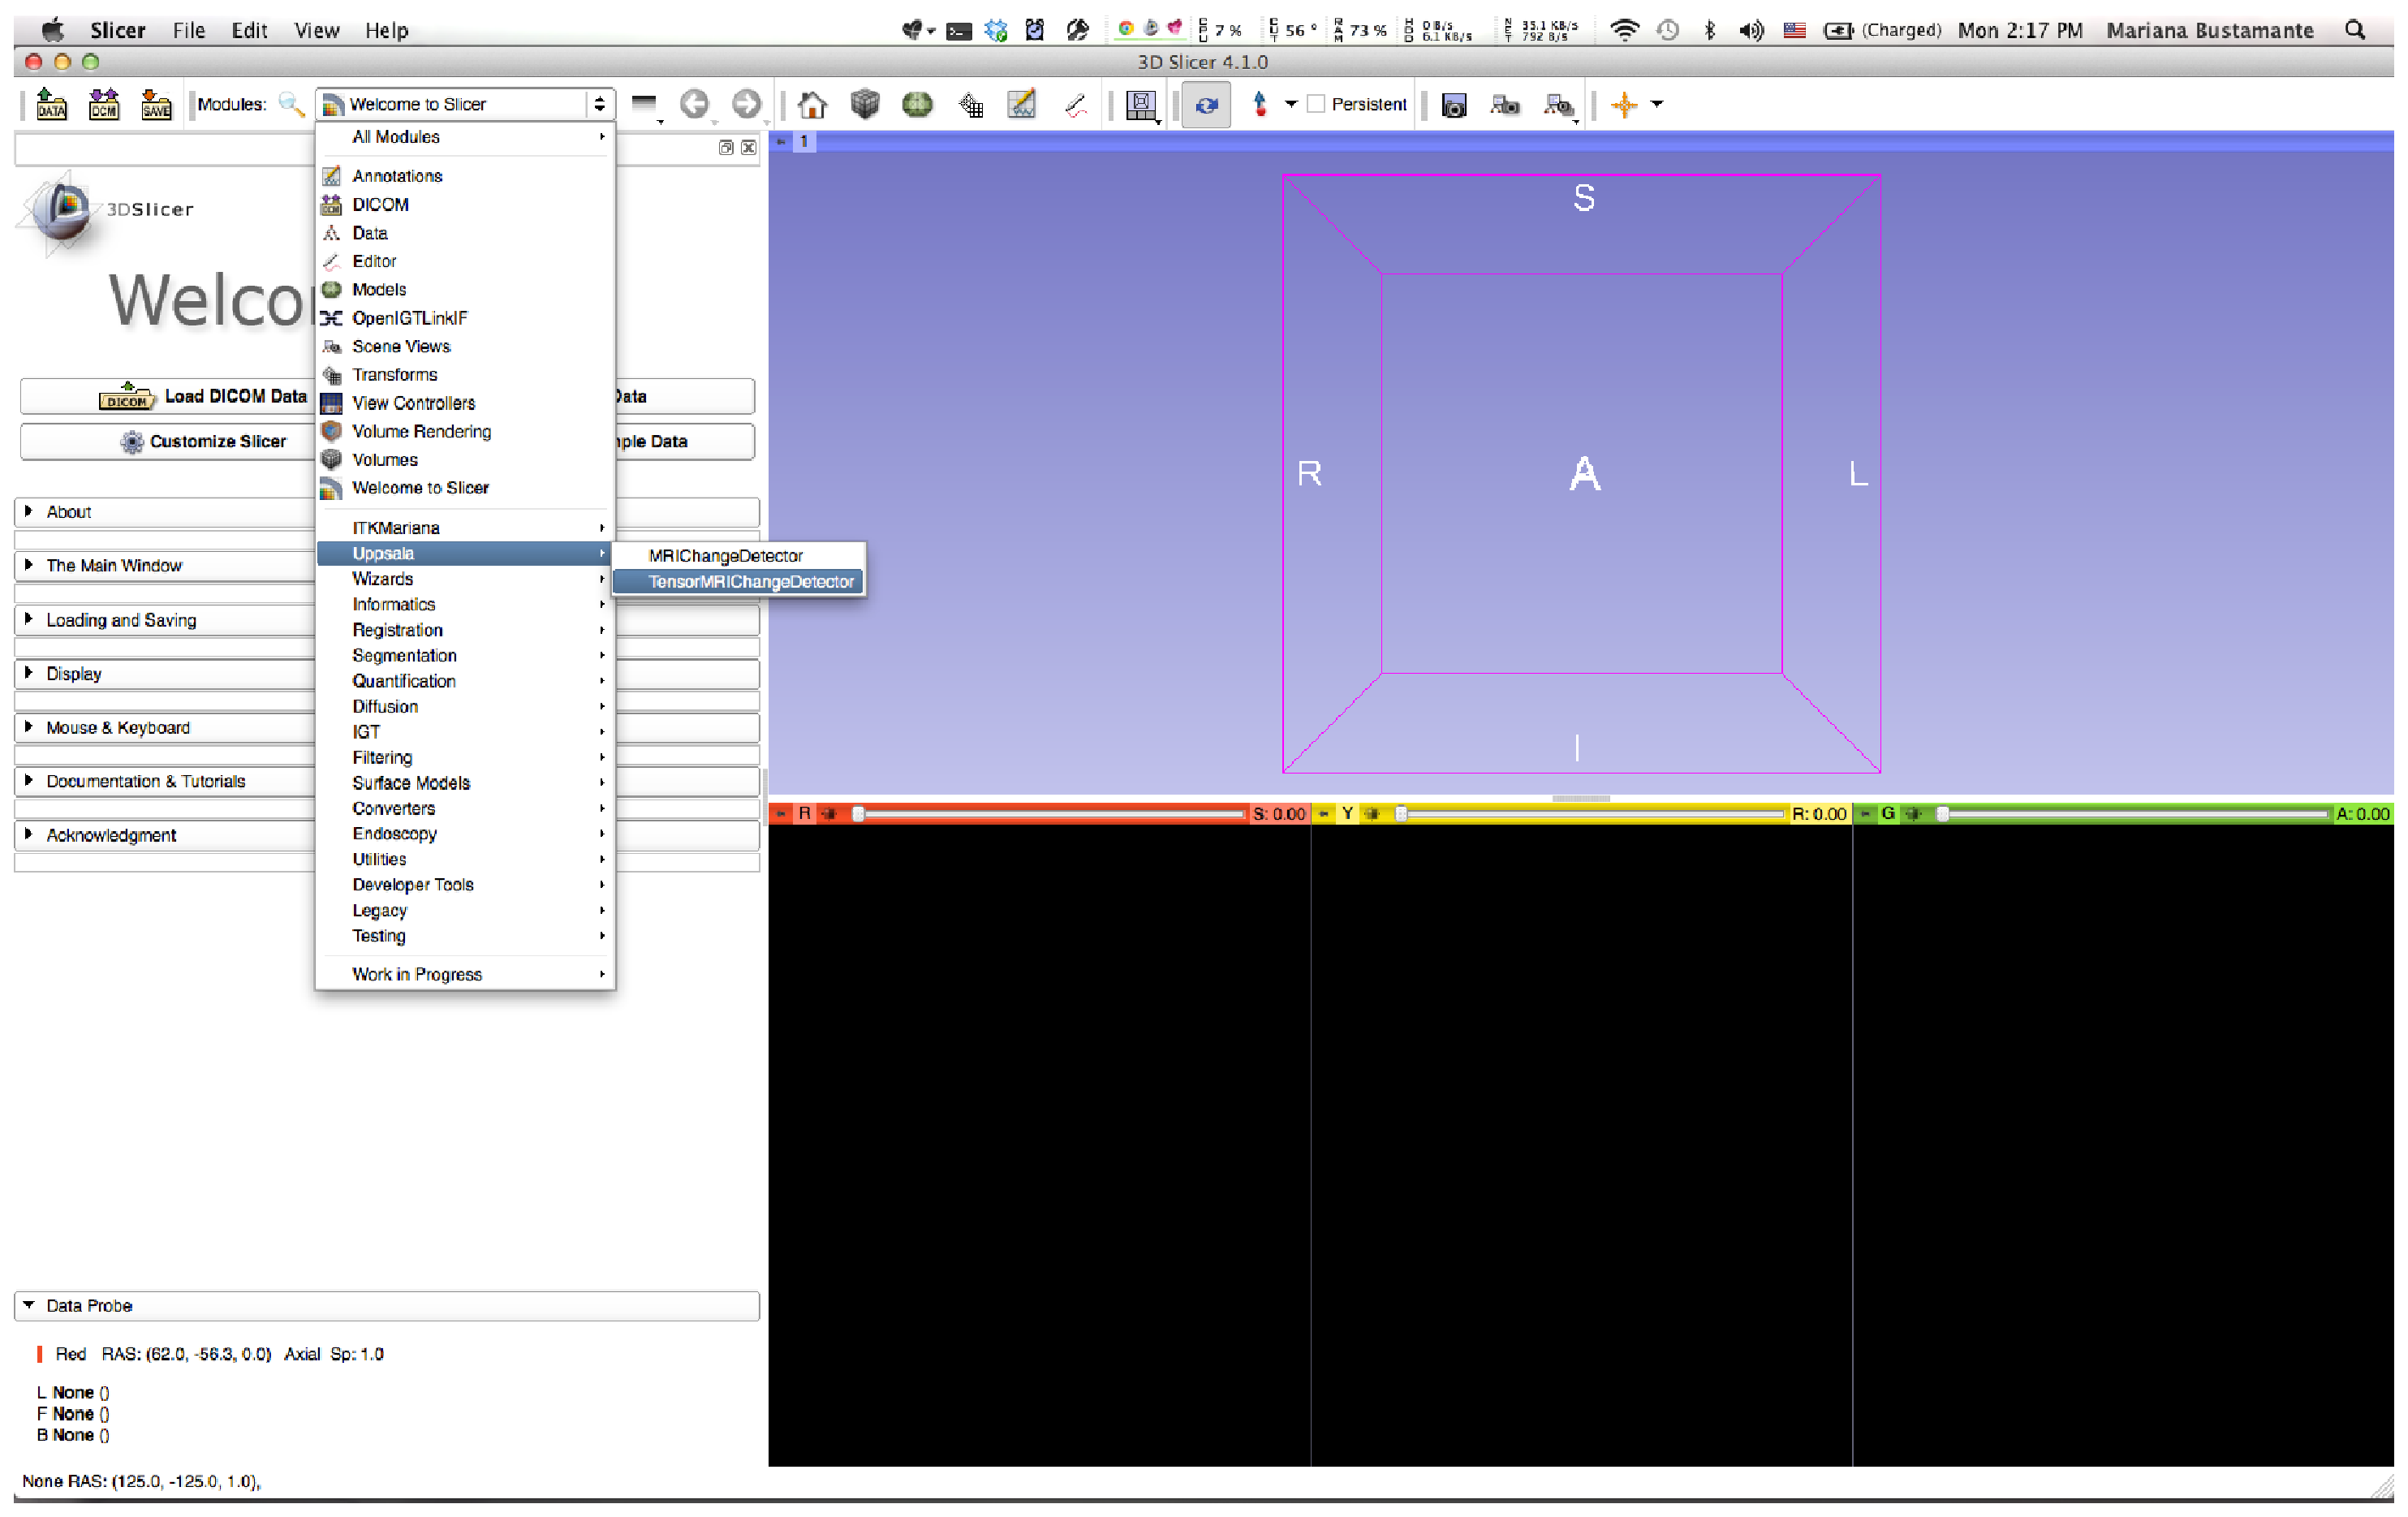
\includegraphics[scale=0.2]{/voxel_example/0.Select.eps}
    \caption{Step 0: Module selection}
    \label{voxel_ex_0}
  \end{figure}
  
\item The user adds the volumes to be analysed.
  
  \begin{figure}[H]
    \centering
    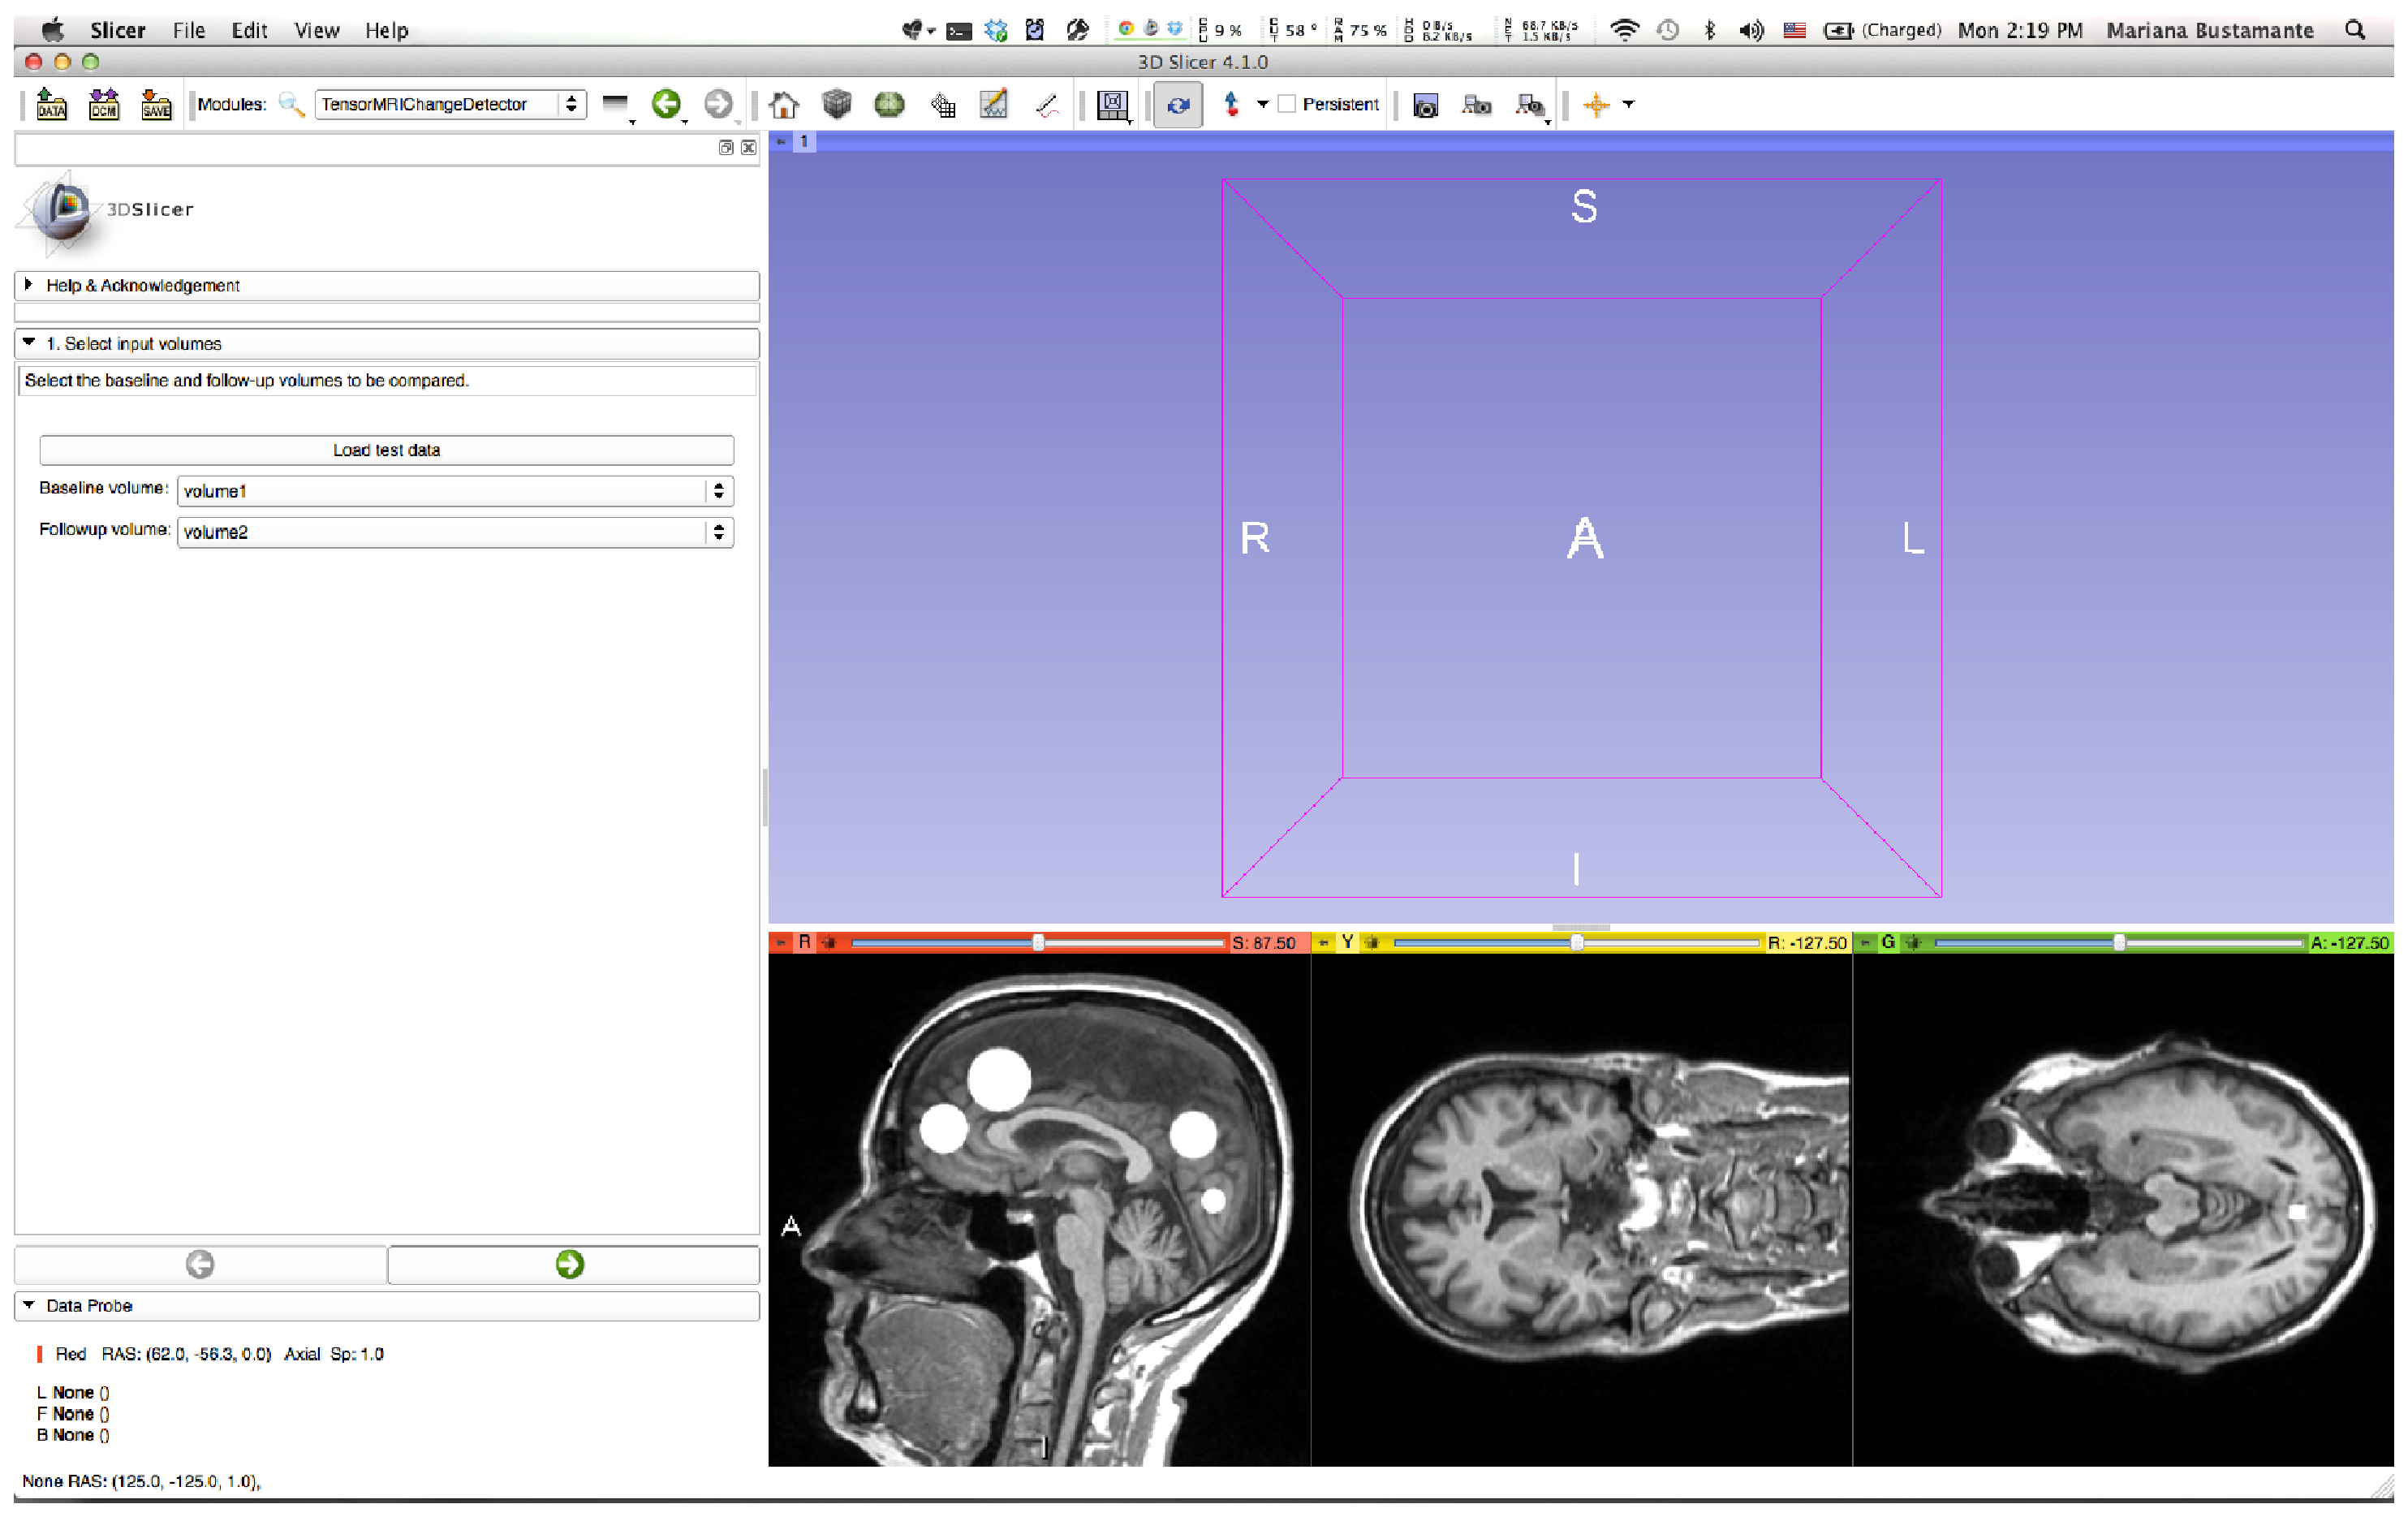
\includegraphics[scale=0.2]{/voxel_example/1.Volumes.eps}
    \caption{Step 1: Adding volumes}
    \label{voxel_ex_1}
  \end{figure}
  
\item The user chooses the registration method to be applied.
  
  \begin{figure}[H]
    \centering
    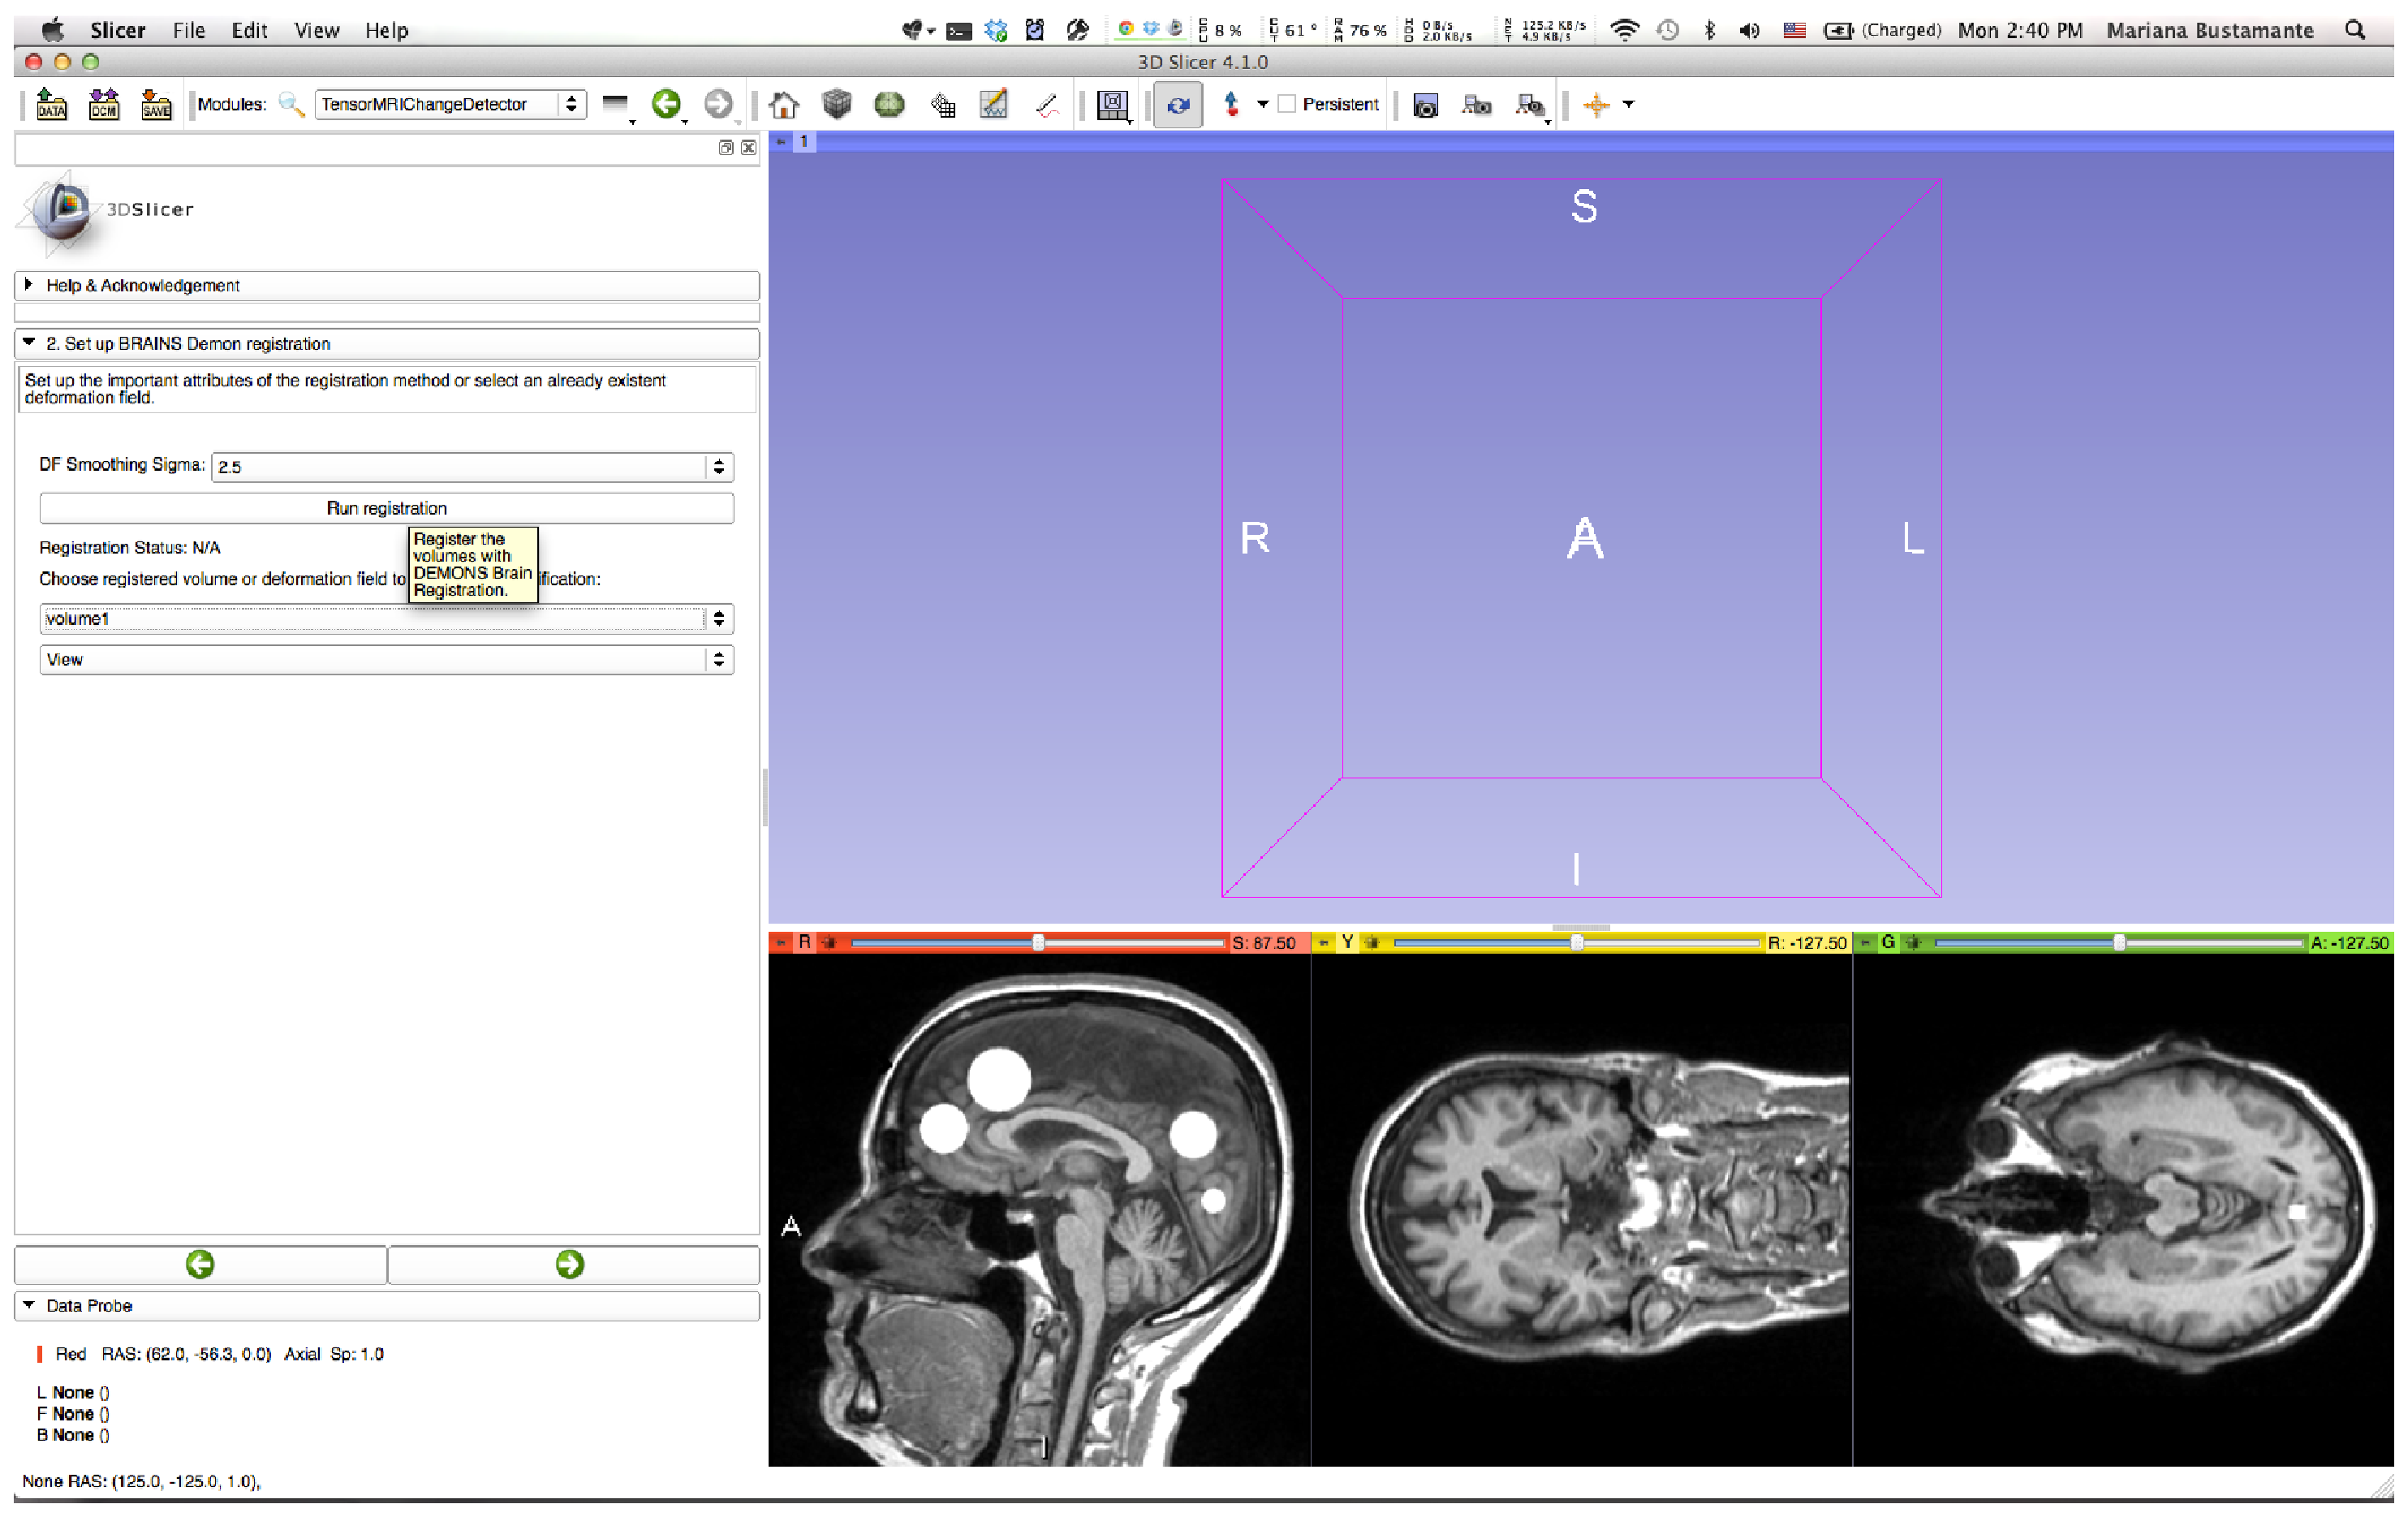
\includegraphics[scale=0.2]{/voxel_example/2.Registration.eps}
    \caption{Step 2: Registration method}
    \label{voxel_ex_2}
  \end{figure}
  
  
\item The user clicks the button ``Run Quantification'' and the
  program runs the subtraction and creation of label volume.
  
  \begin{figure}[H]
    \centering
    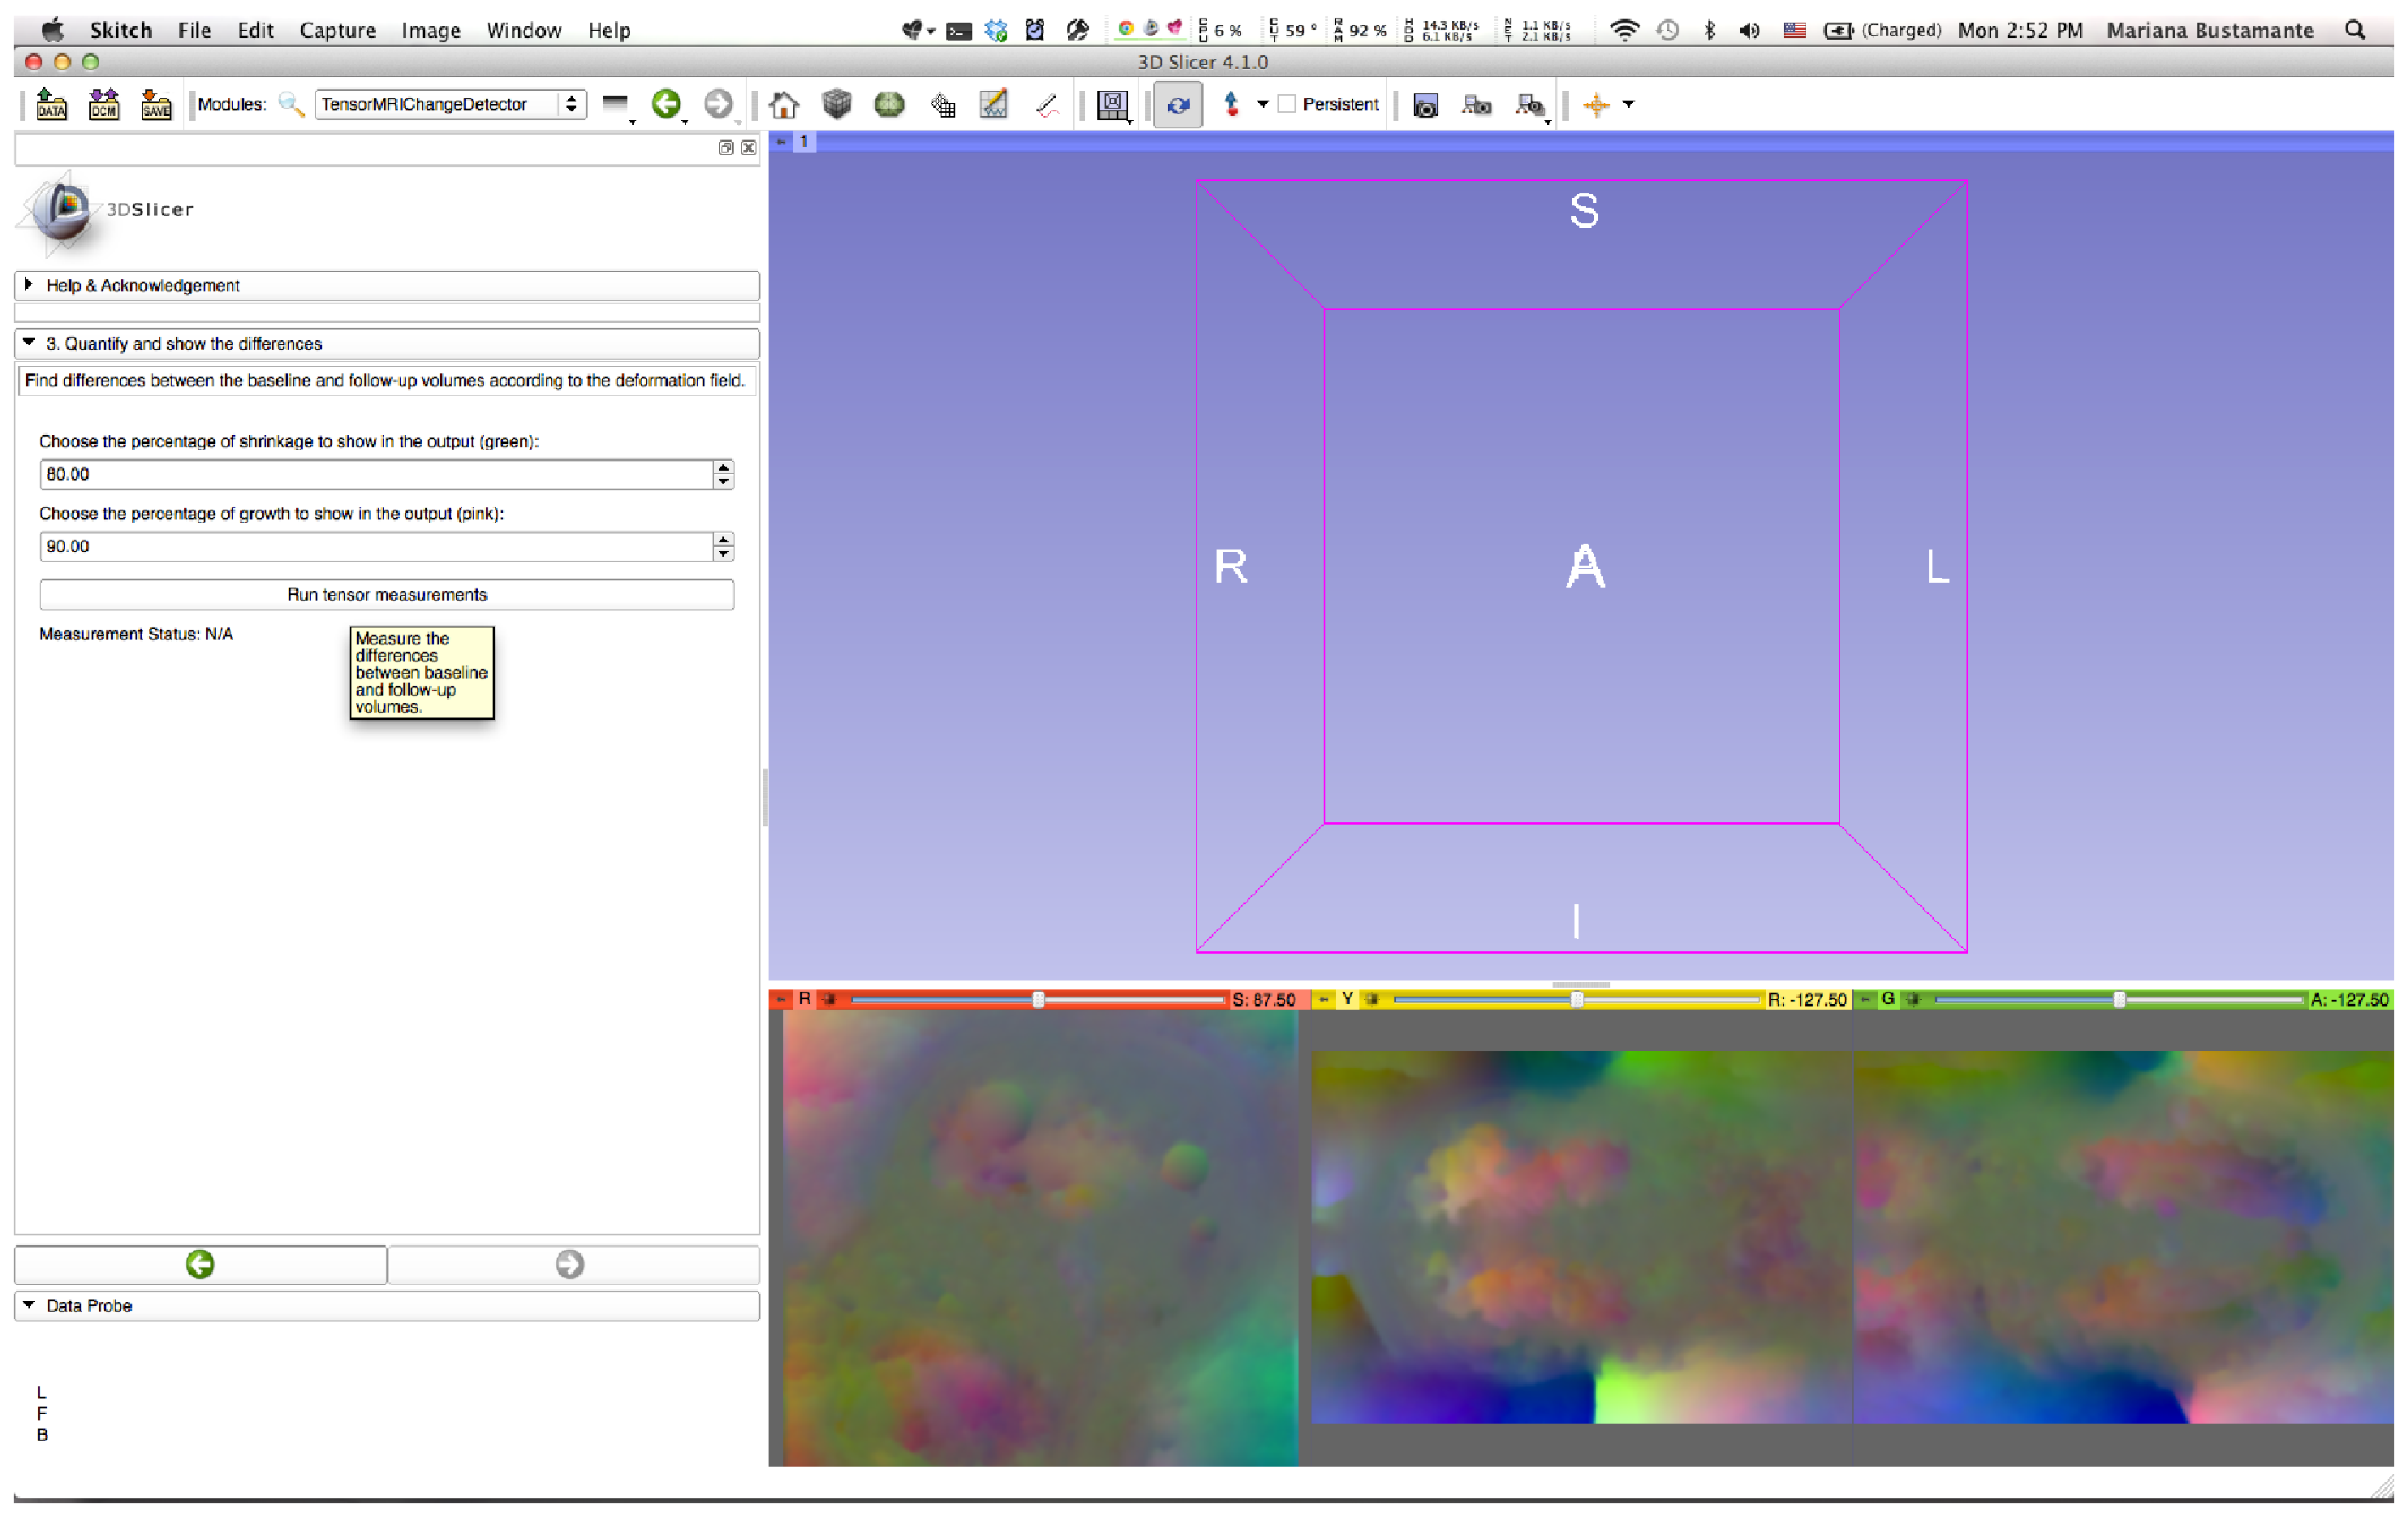
\includegraphics[scale=0.2]{/voxel_example/3.Quantification.eps}
    \caption{Step 3: Running quantification}
    \label{voxel_ex_3}
  \end{figure}
  
\item The program shows the resulting label volume.
  
  \begin{figure}[H]
    \centering
    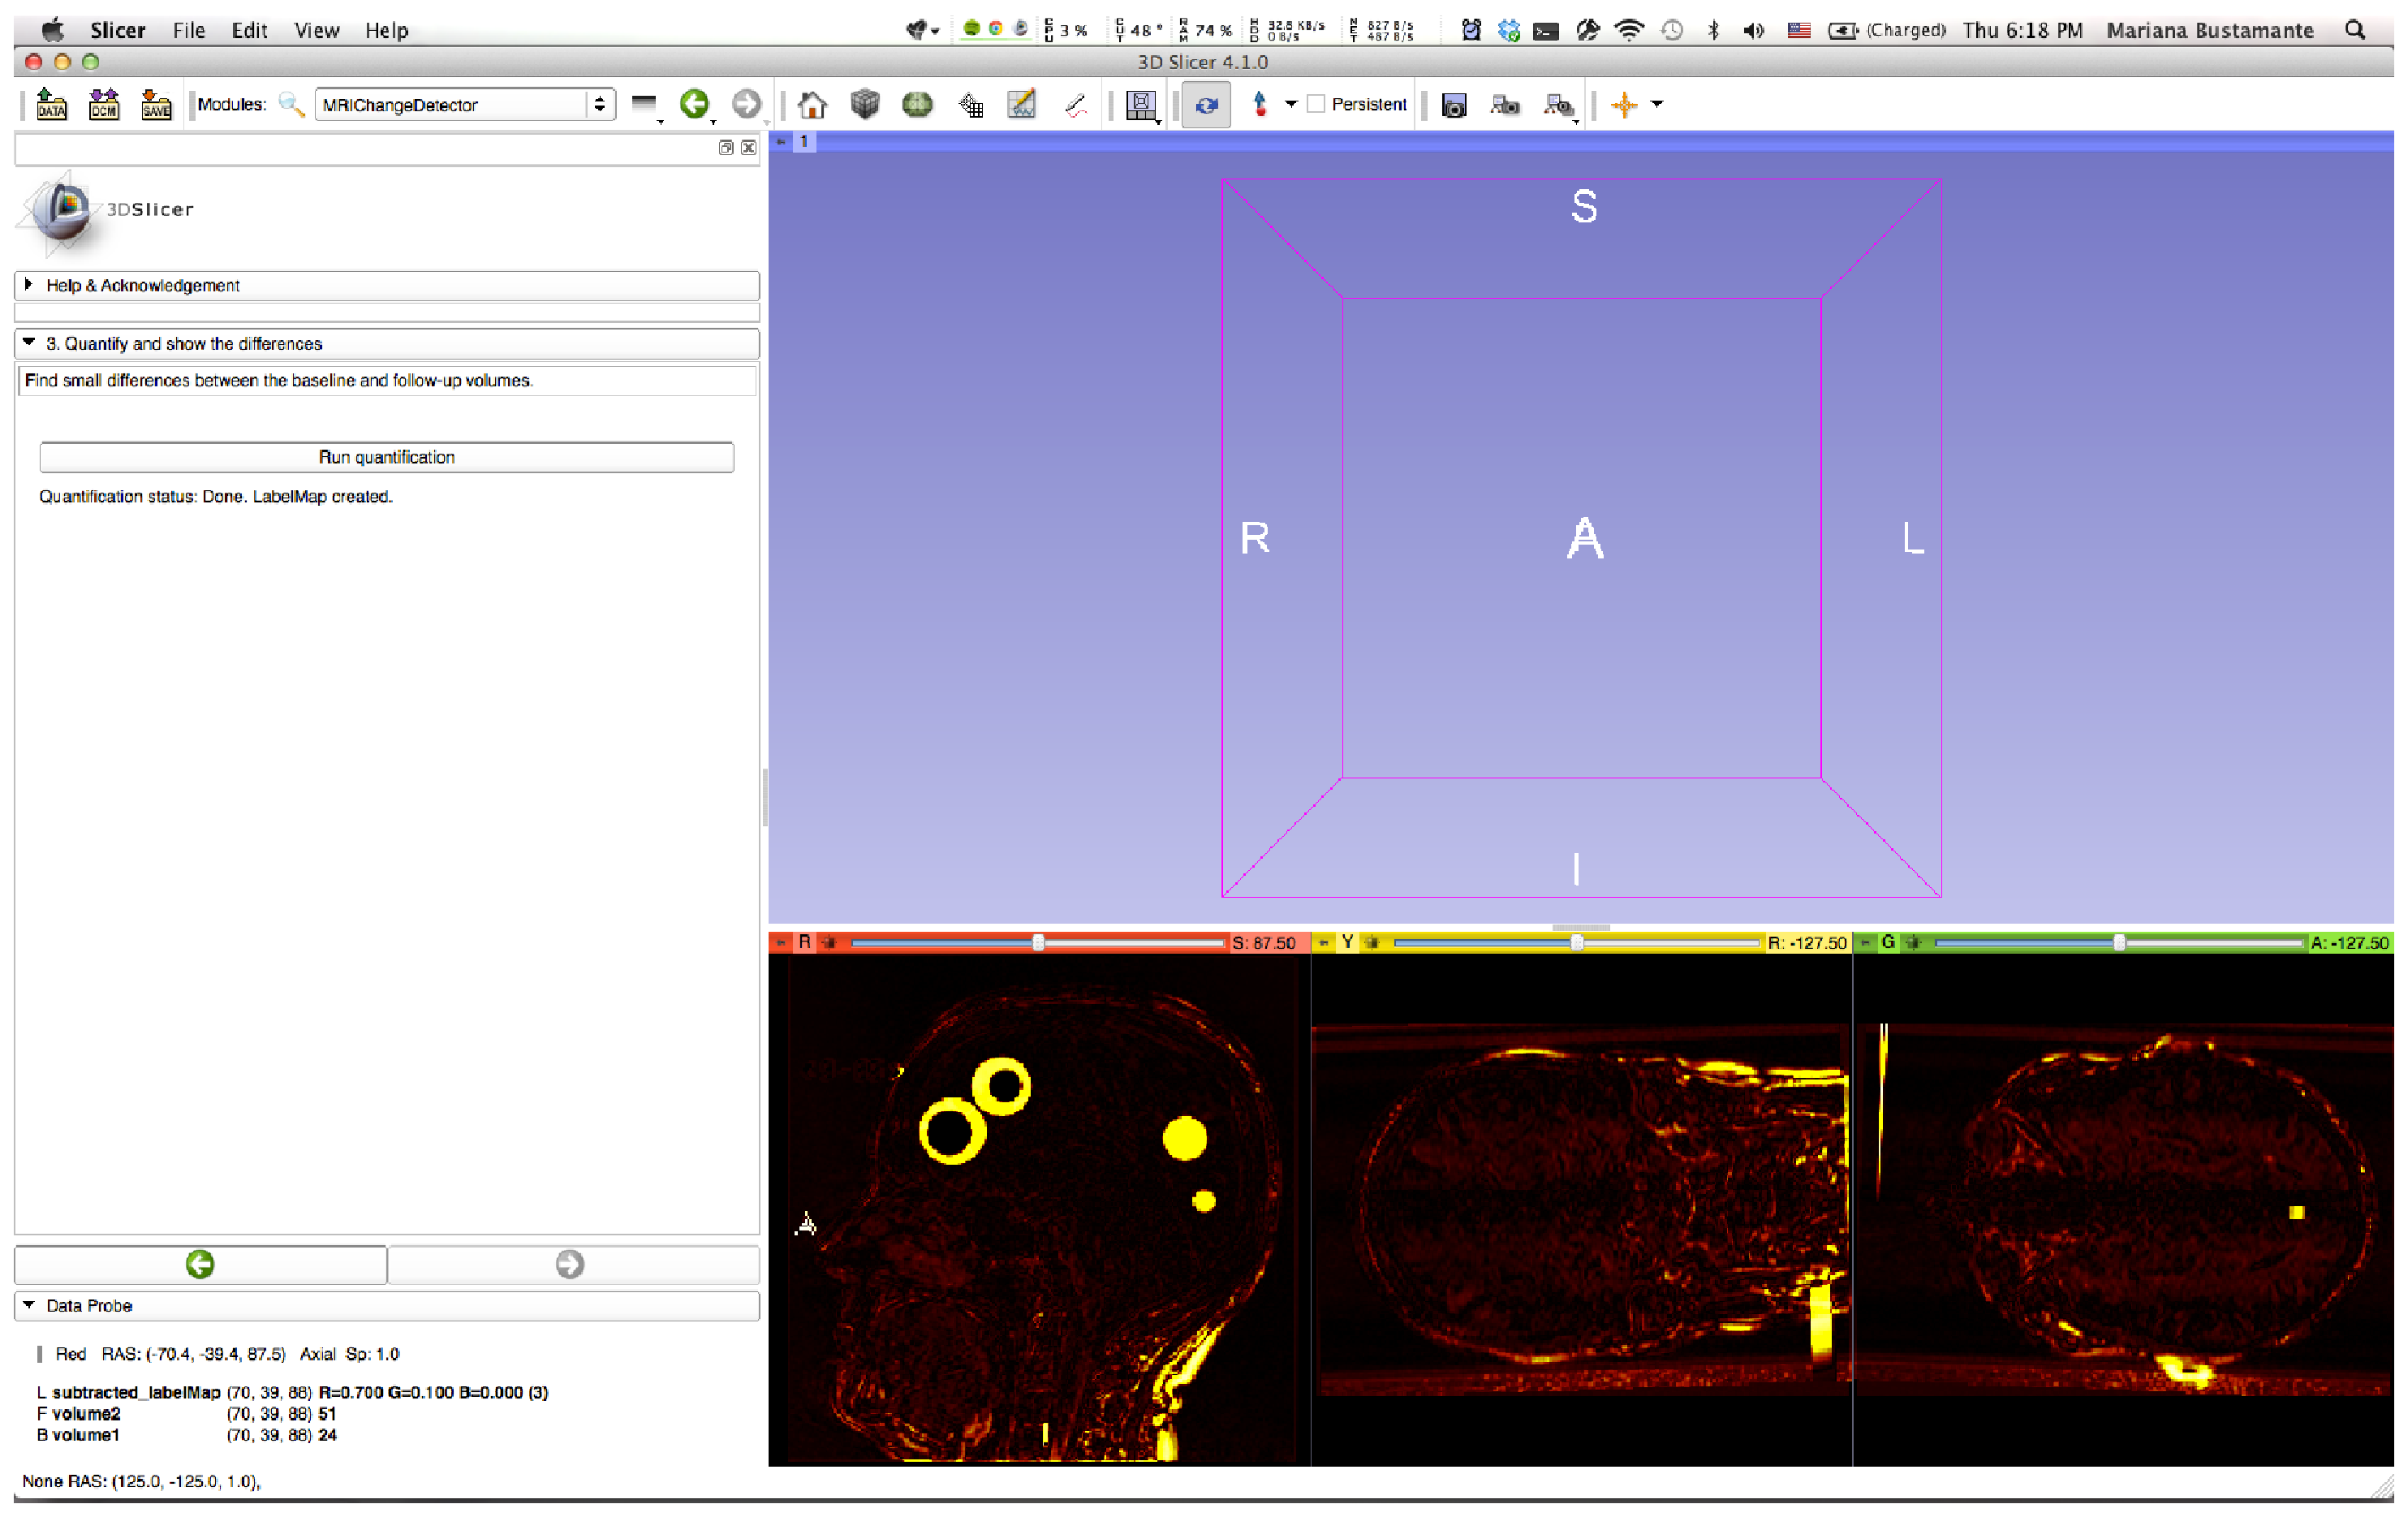
\includegraphics[scale=0.2]{/voxel_example/4.Result1.eps}
    \caption{Step 4: Quantification result}
    \label{voxel_ex_4}
  \end{figure}

  Note that the resulting differences look like rings. This is the
  expected result because both of the original volumes were modified
  by adding circles of distinct sizes.
  
\item The user can now watch the label volume on top of the original
  volume and move the planes as he wishes.
  
  \begin{figure}[H]
    \centering
    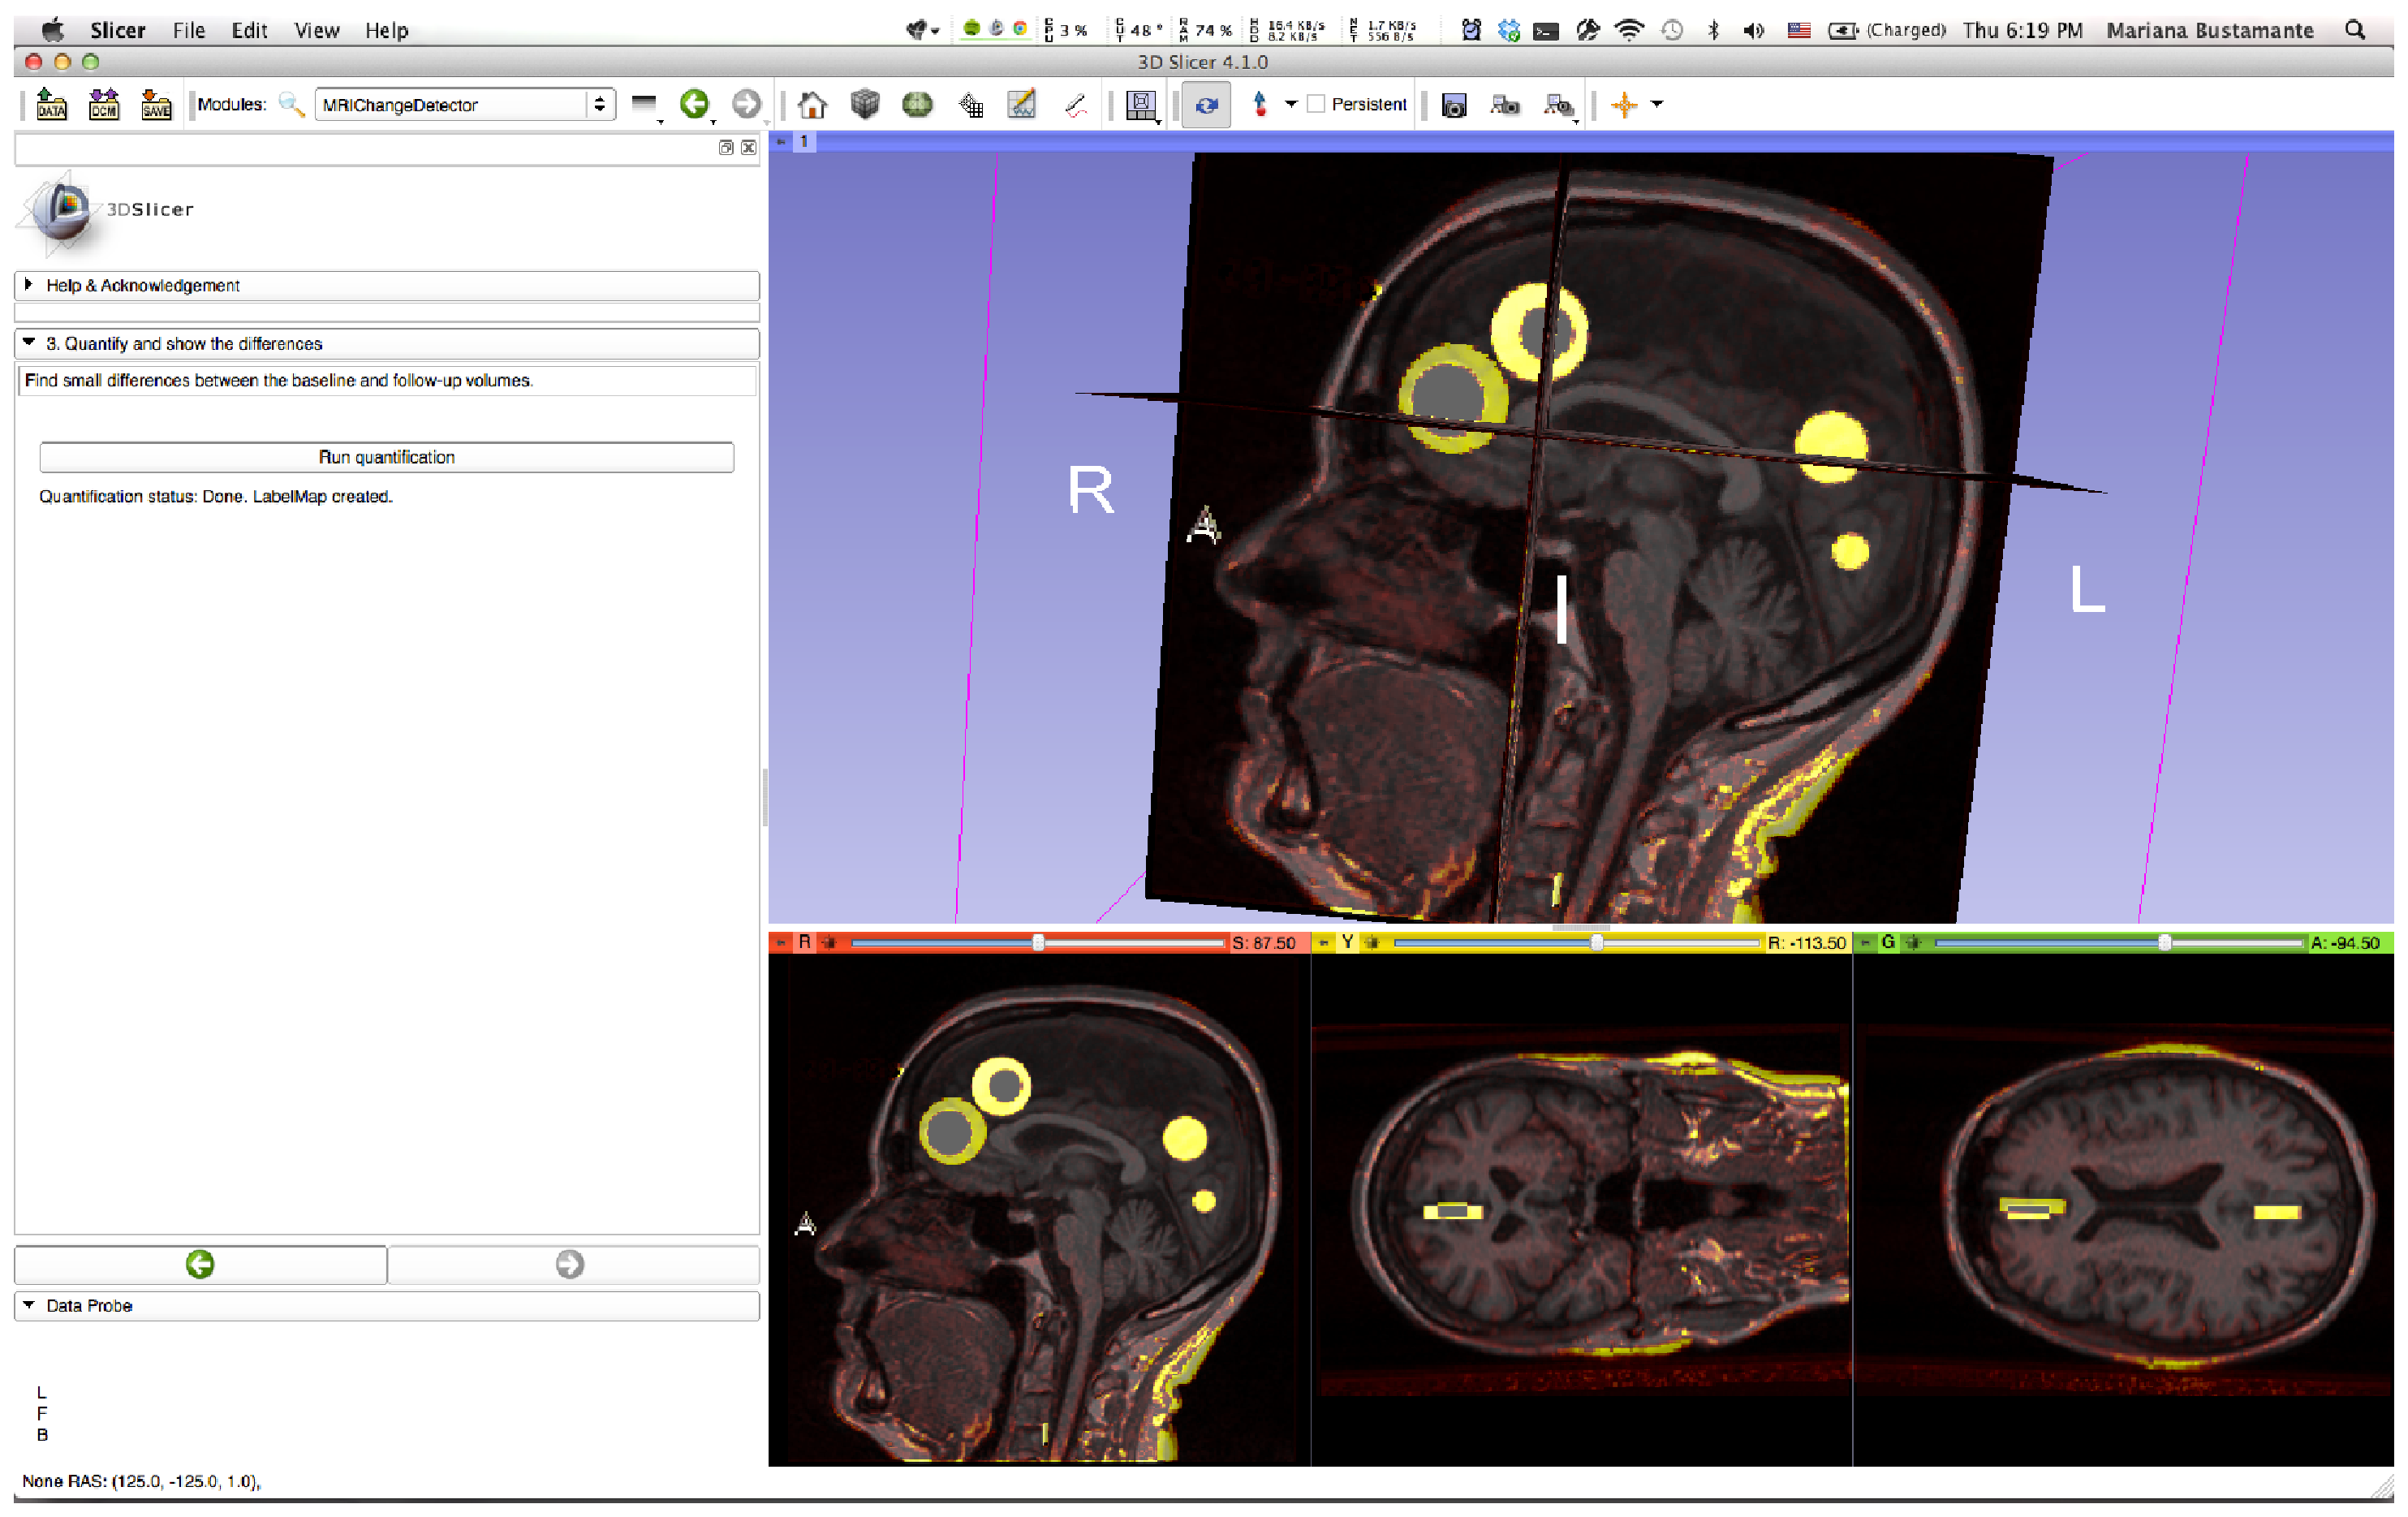
\includegraphics[scale=0.2]{/voxel_example/5.Result2.eps}
    \caption{Step 5: User visualization}
    \label{voxel_ex_5}
  \end{figure}

\end{enumerate}


\subsubsection{Technical Details}
The user interface of the module is written in \textit{Python} using
some libraries from \textit{Qt} and \textit{CTK}, being
\textit{ctkWorkflowWidgetStep} from \textit{CTK} the most important
since it allows the creation of a ``step-by-step'' wizard.\\


The part of the module in charge of the subtraction of volumes is
written in \textit{C++} using \textit{ITK}.

The subtraction is done using the ITK filter
\textit{AbsoluteValueDifferenceImageFilter}, which computes the
difference between each two pixels and then calculates the absolute
value of the result. This allows the module to detect all the possible
differences between the volumes, regardless of the sign of the
resulting values.\\


\subsection{Tensor-based method}



\subsubsection{Strengths and Weaknesses}

\subsubsection{Example}


\subsubsection{Technical Details}